%%%%%%%%%%%%%%%%%%%%%%%%%%%%%%%%%%%%%%%%%
%  My documentation report
%  Objetive: Explain what I did and how, so someone can continue with the investigation
%
% Important note:
% Chapter heading images should have a 2:1 width:height ratio,
% e.g. 920px width and 460px height.
%
%%%%%%%%%%%%%%%%%%%%%%%%%%%%%%%%%%%%%%%%%


%----------------------------------------------------------------------------------------
%	PACKAGES AND OTHER DOCUMENT CONFIGURATIONS
%----------------------------------------------------------------------------------------

\documentclass[11pt,fleqn]{book} % Default font size and left-justified equations

\usepackage[top=3cm,bottom=3cm,left=3.2cm,right=3.2cm,headsep=10pt,letterpaper]{geometry} % Page margins

\usepackage{xcolor} % Required for specifying colors by name
\definecolor{ocre}{RGB}{52,177,201} % Define the orange color used for highlighting throughout the book

% Font Settings
\usepackage{avant} % Use the Avantgarde font for headings
%\usepackage{times} % Use the Times font for headings
\usepackage{mathptmx} % Use the Adobe Times Roman as the default text font together with math symbols from the Symbol, Chancery and Computer Modern fonts
\usepackage{microtype} % Slightly tweak font spacing for aesthetics
\usepackage[utf8]{inputenc} % Required for including letters with accents
\usepackage[T1]{fontenc} % Use 8-bit encoding that has 256 glyphs
\usepackage{amsthm}
\usepackage{clipboard}
\usepackage{graphicx}
\graphicspath{ {./Pictures/} }

% Bibliography
\usepackage[style=alphabetic,sorting=nyt,sortcites=true,autopunct=true,babel=hyphen,hyperref=true,abbreviate=false,backref=true,backend=biber]{biblatex}
\addbibresource{bibliography.bib} % BibTeX bibliography file
\defbibheading{bibempty}{}

\input{structure} % Insert the commands.tex file which contains the majority of the structure behind the template

%----------------------------------------------------------------------------------------
%	Definitions of new commands
%----------------------------------------------------------------------------------------

\def\R{\mathbb{R}}
\newcommand{\cvx}{convex}

\begin{document}

%----------------------------------------------------------------------------------------
%	TITLE PAGE
%----------------------------------------------------------------------------------------

\begingroup
\thispagestyle{empty}
\AddToShipoutPicture*{\put(0,0){\includegraphics[scale=1.25]{narwhal}}} % Image background
\centering
\vspace*{5cm}
\par\normalfont\fontsize{35}{35}\sffamily\selectfont
\textbf{Narwhal}\\
{\LARGE Chess game manipulator}\par % Book title
\vspace*{1cm}
{\Huge Operating Guide}\par % Author name
\endgroup

%----------------------------------------------------------------------------------------
%	COPYRIGHT PAGE
%----------------------------------------------------------------------------------------

\newpage
~\vfill
\thispagestyle{empty}

%\noindent Copyright \copyright\ 2014 Andrea Hidalgo\\ % Copyright notice

\noindent \textsc{Institute of Field Robotics and Automation, King Mongkut's University of Technology Thonburi}\\

% \noindent \textsc{github.com/LaurethTeX/Clustering}\\ % URL

\noindent This project was done under the supervision of Unicorn Tech\\ % License information

\noindent \textit{First release, August 2022} % Printing/edition date

%----------------------------------------------------------------------------------------
%	TABLE OF CONTENTS
%----------------------------------------------------------------------------------------

\chapterimage{narwhal_bar.png} % Table of contents heading image

\pagestyle{empty} % No headers

\tableofcontents % Print the table of contents itself

%\cleardoublepage % Forces the first chapter to start on an odd page so it's on the right

\pagestyle{fancy} % Print headers again

%----------------------------------------------------------------------------------------
%	CHAPTER 1
%----------------------------------------------------------------------------------------

\chapterimage{narwhal_bar2.png} % Chapter heading image
\chapter{Chessboard State Estimation and Chess AI}
\section{Environment Initialization}
\subsection{Initialize environment}
All softwares (except low-level control) were written as nodes in \textbf{module89} ROS2 package which located at \texttt{/home/fiborobotlab/dev\_ws/src}.
ROS2 environment automatically intialized each time when new section is opened by several commands inside \texttt{/home/fiborobotlab/.bashrc}, thus you don't need to source ROS2 installation. However, you still need to source the package installation before run or launch node(s) inside the package, this can be done in 2 ways.\\
Using standard \texttt{bash} command with setup script.\\
\texttt{>> bash /home/fiborobotlab/dev\_ws/install/setup.bash}\\
\\
Or use shorter command written in alias.\\
\texttt{>> ins}\\
\\
Use this command to run all nodes at once \\
\texttt{>> ros2 launch module89 main.launch.py}\\

\section{Camera Setup}
\subsection{Camera Installation}
Install single RGB camera above target chessboard and face down toward target chessboard with resolution of 1080p (1920x1080 pixels). Make sure target chessboard is inside camera frame, side-alignment is unnecessary (software can perform auto-alignment after calibration). We use camera coordinate as diagram below

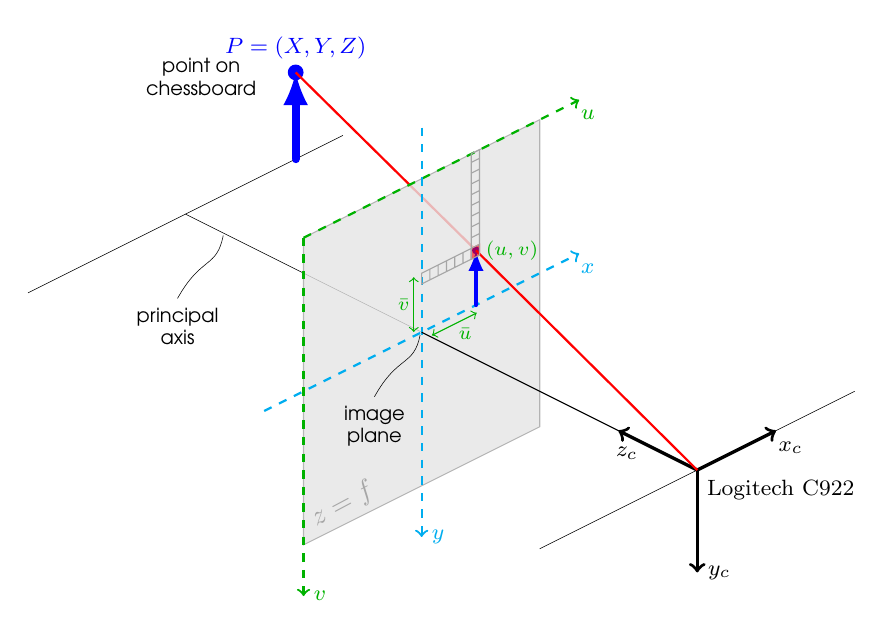
\begin{tikzpicture}

\usetikzlibrary{calc}

% Picture's vectors definition
\def\xOne{1}
\def\xTwo{0.5}
\def\yOne{0}
\def\yTwo{-1.3}
\def\zOne{-1}
\def\zTwo{0.5}

% CAMERA COORDINATE SYSTEM
%\draw[thick,->] (0,0) -- (\xOne,\xTwo) node[anchor=north]{$x$};
%\draw[thick,->] (0,0) -- (\yOne,\yTwo) node[anchor=west]{$y$};
%\draw[thick,->] (0,0) -- (\zOne,\zTwo) node[anchor=north,yshift=-2pt,xshift=3pt]{$z$};
\draw[very thick,->] (-\zOne/2,-\zTwo/2) -- (-\zOne/2+\xOne,-\zTwo/2+\xTwo) node[anchor=north west, xshift=-3pt,font=\footnotesize]{$x_c$};
\draw[very thick,->] (-\zOne/2,-\zTwo/2) -- (-\zOne/2+\yOne,-\zTwo/2+\yTwo) node[anchor=west,font=\footnotesize]{$y_c$};
\draw[very thick,->] (-\zOne/2,-\zTwo/2) -- (\zOne/2,\zTwo/2) node[anchor=north,yshift=-2pt,xshift=3pt,font=\footnotesize]{$z_c$};
\draw (-\zOne/2,-\zTwo/2) node[anchor=north west,font=\footnotesize]{Logitech C922};

% CAMERA AXIS ELONGATION
\draw[very thin,solid] (-\zOne/2-2*\xOne,-\zTwo/2-2*\xTwo) -- (-\zOne/2+2*\xOne,-\zTwo/2+2*\xTwo); % x elongation
\draw[very thin,solid] (3*\zOne,3*\zTwo) -- (6*\zOne,6*\zTwo); % optical axis behind projection plane

% REFERENCE LINES
%\draw[thin,dashed] (1.4*\xOne-\zOne/2,1.4*\xTwo-\zTwo/2) -- (6*\zOne+1.4*\xOne,6*\zTwo+1.4*\xTwo); % object x position
\draw[very thin,solid] (6*\zOne-2*\xOne,6*\zTwo-2*\xTwo) -- (6*\zOne+2*\xOne,6*\zTwo+2*\xTwo) node[anchor=west]{}; %object z position

% WORLD OBJECT
\draw[-latex,line width=3pt,blue,line cap=round] (6*\zOne+1.4*\xOne,6*\zTwo+1.4*\xTwo) -- (6*\zOne+1.4*\xOne,6*\zTwo+1.4*\xTwo+1.1) node[anchor=south,font=\footnotesize]{$ P = (X,Y,Z) $};
\node[circle,inner sep=0pt,minimum size=0.2cm,fill=blue] (object) at (6*\zOne+1.4*\xOne,6*\zTwo+1.4*\xTwo+1.1) {};
% \draw[very thin] (3*\zOne-0.02*\xOne+0.02*\yOne,3*\zTwo-0.02*\xTwo+0.02*\yTwo) .. controls (3*\zOne-0.1*\xOne+0.3*\yOne,3*\zTwo-0.1*\xTwo+0.3*\yTwo) and (3*\zOne-0.3*\xOne+0.1*\yOne,3*\zTwo-0.3*\xTwo+0.1*\yTwo) ..  (3*\zOne-0.6*\xOne+0.4*\yOne,3*\zTwo-0.6*\xTwo+0.4*\yTwo)
\node[anchor=north,align=center,font=\sffamily\scriptsize](object) at (5.8*\zOne+0.0*\xOne,5.8*\zTwo+0.0*\xTwo+2.2) {point on\\chessboard};

% PROJECTION LINE BEHIND PROJECTION PLANE
\draw[thick,solid,red] (3*\zOne+0.69*\xOne,3*\zTwo+0.7*\xTwo+0.69) -- (6*\zOne+1.4*\xOne,6*\zTwo+1.4*\xTwo+1.1);

%% PROJECTION PLANE
\filldraw[fill=gray!20,draw=gray!70,opacity=0.8] (3*\zOne-1.5*\xOne-1.5*\yOne,3*\zTwo-1.5*\xTwo-1.5*\yTwo) -- (3*\zOne+1.5*\xOne-1.5*\yOne,3*\zTwo+1.5*\xTwo-1.5*\yTwo) -- (3*\zOne+1.5*\xOne+1.5*\yOne,3*\zTwo+1.5*\xTwo+1.5*\yTwo) -- (3*\zOne-1.5*\xOne+1.5*\yOne,3*\zTwo-1.5*\xTwo+1.5*\yTwo) -- (3*\zOne-1.5*\xOne-1.5*\yOne,3*\zTwo-1.5*\xTwo-1.5*\yTwo);

% PLOJECTION PLANE COORDINATE SYSTEM u,v
\draw[->,thick,green!70!black,dashed] (3*\zOne-1.5*\xOne-1.5*\yOne,3*\zTwo-1.5*\xTwo-1.5*\yTwo) -- (3*\zOne+2*\xOne-1.5*\yOne,3*\zTwo+2*\xTwo-1.5*\yTwo)
     node[anchor=north west, xshift=-3pt,font=\footnotesize]{$u$};
\draw[->,thick,green!70!black,dashed] (3*\zOne-1.5*\xOne-1.5*\yOne,3*\zTwo-1.5*\xTwo-1.5*\yTwo) -- (3*\zOne-1.5*\xOne-1.5*\yOne,3*\zTwo-1.5*\xTwo+2*\yTwo)
     node[anchor=west,font=\footnotesize]{$v$};

% PROJECTION PLANE COORDINATE SYSTEM x,y
\draw[->,thick,cyan,dashed] (3*\zOne-2*\xOne,3*\zTwo-2*\xTwo) -- (3*\zOne+2*\xOne,3*\zTwo+2*\xTwo)
     node[anchor=north west, xshift=-3pt,font=\footnotesize]{$x$};
\draw[->,thick,cyan,dashed] (3*\zOne-2*\yOne,3*\zTwo-2*\yTwo) -- (3*\zOne+2*\yOne,3*\zTwo+2*\yTwo)
     node[anchor=west,font=\footnotesize]{$y$};

% PROJECTION  OBJECT
\draw[-latex,line width=1.5pt,blue,line cap=round] (3*\zOne+0.69*\xOne,3*\zTwo+0.69*\xTwo) -- (3*\zOne+0.69*\xOne,3*\zTwo+0.69*\xTwo+0.69);
\node[circle,inner sep=0pt,minimum size=0.1cm,fill=blue] (object) at (3*\zOne+0.69*\xOne,3*\zTwo+0.7*\xTwo+0.69) {};

% PIXEL OBJECT
\filldraw[red,opacity=0.6] (3*\zOne+6*0.105*\xOne,3*\zTwo+0.75+6*0.105*\xTwo) -- ++(0.105*\xOne,0.105*\xTwo) -- ++(0.105*\yOne,0.105*\yTwo) -- ++(-0.105*\xOne,-0.105*\xTwo) -- ++(-0.105*\yOne,-0.105*\yTwo);

% PROJECTION LINE IN FRONT OF PROJECTION PLANE
\draw[thick,solid,red] (-\zOne/2,-\zTwo/2) -- (3*\zOne+0.69*\xOne,3*\zTwo+0.7*\xTwo+0.69);

% OPTICAL AXIS IN FRONT OF PROJECTION PLANE
\draw[thin,solid] (0,0) -- (3*\zOne,3*\zTwo);

% ANNOTATIONS
% z = f
\draw (3*\zOne-1*\xOne+1.3*\yOne,3*\zTwo-1*\xTwo+1.3*\yTwo) node[gray!70,rotate=28] {$ z = f $};
% bar(u)
\draw[to-to, green!70!black] (3*\zOne+0.13*\xOne+0.08*\yOne,3*\zTwo+0.13*\xTwo+0.08*\yTwo) -- (3*\zOne+0.7*\xOne+0.08*\yOne,3*\zTwo+0.7*\xTwo+0.08*\yTwo) node[midway,anchor=north west,xshift=-2pt,yshift=2pt,font=\scriptsize] {$ \bar{u} $};
% bar(v)
\draw[to-to, green!70!black] (3*\zOne-0.1*\xOne-0.04*\yOne,3*\zTwo-0.1*\xTwo-0.04*\yTwo) -- (3*\zOne-0.1*\xOne,3*\zTwo-0.1*\xTwo+0.75) node[midway,anchor=east,xshift=2pt,font=\scriptsize] {$ \bar{v} $};
% (u,v)
\node[green!70!black,anchor=west,font=\scriptsize] at (3*\zOne+0.69*\xOne,3*\zTwo+0.7*\xTwo+0.69) {$ (u,v) $};
% principal point
\draw[very thin] (3*\zOne-0.02*\xOne+0.02*\yOne,3*\zTwo-0.02*\xTwo+0.02*\yTwo) .. controls (3*\zOne-0.1*\xOne+0.3*\yOne,3*\zTwo-0.1*\xTwo+0.3*\yTwo) and (3*\zOne-0.3*\xOne+0.1*\yOne,3*\zTwo-0.3*\xTwo+0.1*\yTwo) ..  (3*\zOne-0.6*\xOne+0.4*\yOne,3*\zTwo-0.6*\xTwo+0.4*\yTwo) node[anchor=north,align=center,font=\sffamily\scriptsize] {image\\plane};
% optical axis
\draw[very thin] (5.5*\zOne-0.02*\xOne+0.02*\yOne,5.5*\zTwo-0.02*\xOne+0.02*\yOne) .. controls (5.5*\zOne-0.1*\xOne+0.3*\yOne,5.5*\zTwo-0.1*\xTwo+0.3*\yTwo) and (5.5*\zOne-0.3*\xOne+0.1*\yOne,5.5*\zTwo-0.3*\xTwo+0.1*\yTwo) ..  (5.5*\zOne-0.6*\xOne+0.4*\yOne,5.5*\zTwo-0.6*\xTwo+0.4*\yTwo) node[anchor=north,align=center,font=\sffamily\scriptsize] {principal\\axis};

% PIXEL POSITION
\draw[thin,gray!70] (3*\zOne,3*\zTwo+0.75) -- ++(0.105*\xOne,0.105*\xTwo) -- ++(0.105*\yOne,0.105*\yTwo) -- ++(-0.105*\xOne,-0.105*\xTwo) -- ++(-0.105*\yOne,-0.105*\yTwo) -- ++(0.21*\xOne,0.21*\xTwo) -- ++(0.105*\yOne,0.105*\yTwo) -- ++(-0.105*\xOne,-0.105*\xTwo) -- ++(-0.105*\yOne,-0.105*\yTwo) -- ++(0.21*\xOne,0.21*\xTwo) -- ++(0.105*\yOne,0.105*\yTwo) -- ++(-0.105*\xOne,-0.105*\xTwo) -- ++(-0.105*\yOne,-0.105*\yTwo) -- ++(0.21*\xOne,0.21*\xTwo) -- ++(0.105*\yOne,0.105*\yTwo) -- ++(-0.105*\xOne,-0.105*\xTwo) -- ++(-0.105*\yOne,-0.105*\yTwo) -- ++(0.21*\xOne,0.21*\xTwo) -- ++(0.105*\yOne,0.105*\yTwo) -- ++(-0.105*\xOne,-0.105*\xTwo) -- ++(-0.105*\yOne,-0.105*\yTwo) -- ++(0.21*\xOne,0.21*\xTwo) -- ++(0.105*\yOne,0.105*\yTwo) -- ++(-0.105*\xOne,-0.105*\xTwo) -- ++(-0.105*\yOne,-0.105*\yTwo) -- ++(0.21*\xOne,0.21*\xTwo) -- ++(0.105*\yOne,0.105*\yTwo) -- ++(-0.105*\xOne,-0.105*\xTwo) -- ++(-0.21*\yOne,-0.21*\yTwo) -- ++(0.105*\xOne,0.105*\xTwo) -- ++(0.105*\yOne,0.105*\yTwo) -- ++(-0.105*\xOne,-0.105*\xTwo) -- ++(-0.21*\yOne,-0.21*\yTwo) -- ++(0.105*\xOne,0.105*\xTwo) -- ++(0.105*\yOne,0.105*\yTwo) -- ++(-0.105*\xOne,-0.105*\xTwo) -- ++(-0.21*\yOne,-0.21*\yTwo) -- ++(0.105*\xOne,0.105*\xTwo) -- ++(0.105*\yOne,0.105*\yTwo) -- ++(-0.105*\xOne,-0.105*\xTwo) -- ++(-0.21*\yOne,-0.21*\yTwo) -- ++(0.105*\xOne,0.105*\xTwo) -- ++(0.105*\yOne,0.105*\yTwo) -- ++(-0.105*\xOne,-0.105*\xTwo) -- ++(-0.21*\yOne,-0.21*\yTwo) -- ++(0.105*\xOne,0.105*\xTwo) -- ++(0.105*\yOne,0.105*\yTwo) -- ++(-0.105*\xOne,-0.105*\xTwo) -- ++(-0.21*\yOne,-0.21*\yTwo) -- ++(0.105*\xOne,0.105*\xTwo) -- ++(0.105*\yOne,0.105*\yTwo) -- ++(-0.105*\xOne,-0.105*\xTwo) -- ++(-0.21*\yOne,-0.21*\yTwo) -- ++(0.105*\xOne,0.105*\xTwo) -- ++(0.105*\yOne,0.105*\yTwo) -- ++(-0.105*\xOne,-0.105*\xTwo) -- ++(-0.21*\yOne,-0.21*\yTwo) -- ++(0.105*\xOne,0.105*\xTwo) -- ++(0.105*\yOne,0.105*\yTwo) -- ++(-0.105*\xOne,-0.105*\xTwo) -- ++(-0.19*\yOne,-0.19*\yTwo) -- ++(0.105*\xOne,0.105*\xTwo) -- ++(0.105*\yOne,0.105*\yTwo);
\end{tikzpicture}
\begin{figure}[h!]
\caption{Camera coordinate used in Narwhal project}
\end{figure}

\subsection{Camera Calibration}
Default camera intrinsic matrix and distortion coefficients is for Logitech C922 USB camera. When change the camera, you need to modify these values at \texttt{package://config/camera\_config.json} for new installed camera.

\subsubsection{Chessboard Pose Calibration \& Color Clustering Lock}
Source package when open new terminal to include module89 in the environment.\\
\\
\texttt{>> ins}\\
\\
Next, run \texttt{chessboard estimator} node to begin calibration of chessboard using command:\\
\\
\texttt{>> ros2 run module89 chessboard\_estimator.py}\\
\\
If camera is connected correctly, this window will opened and begin streaming automatically at 720p (scaled down from 1080p) along with several buttons as in Figure \ref{fig:GUI_camera}. After each installation or camera displaced, the chessboard pose matrix might be changed, so new calibration might be done by\\
\begin{itemize}
    \item Click at 4 corners of chessboard (regarding black/white side bar).
    \item If you mistaken click any point other than chessboard corner, you can use \textbf{Clear Points} button to reset point(s) stored in buffer.
    \item Make sure you click exactly 4 points (any other amount of point will not be accepted by auto-calibration function and nothing will happen) before press \textbf{Confirm} button to confirm and apply selections. This node will use these 4 points with \texttt{solvePnP()} along with some image processing to estimate aligned pose of chessboard.
    \item Applied corners will only stored in memory, press \textbf{Save} button if you want to store calibration for later use without 4 points input again.
    \item By clicking \textbf{Load} button, saved calibration will restored from disk if exist. If nothing has moved after most recent calibration, this is the only button you need to press after run this node.
    \item After chessboard is perfectly aligned in GUI, the system will beginning clustering process automatically then press \textbf{LOCK Color clustering} button to stop updating the model and lock color which most of them near corresponding side (note: this button can be toggle to unlock-relock)
    
\end{itemize}
% \includegraphics{GUI_camera}
\begin{figure}
\centering
\includegraphics[width=0.8\textwidth]{GUI_camera}
\caption{\label{fig:GUI_camera}GUI for chessboard pose calibration written by Qt5}
% \fig[0.5]{GUI_camera.png}{GUI for chessboard pose calibration written by Qt5}{GUI_camera}
\end{figure}

\subsection{Chessboard tile preparation}
Before feeding image to classification model, we have to preprocess them to a Tensor with shape (64, 32, 32, 3) which is 3 channel images with size 32x32 using fixed batchsize of 64. Thus, we need to divide raw image for each tile, resize, and zero-pad chessboard tile.

\section{AI (Vision)}
\subsection{Chess piece classification}
\raggedright
We use only one lightweight-CNNs based classification model created with \textbf{TensorFlow2} and optimized by \href{https://docs.openvino.ai/latest/index.html}{OpenVINO} which be able to run on \textbf{\color{blue} Intel UHD Graphics Xe G4 48EUs} via \textbf{OpenCL} using \href{https://docs.openvino.ai/latest/openvino_docs_install_guides_install_runtime.html}{\textbf{OpenVINO runtime}} at \textbf{\color{blue}>200fps}. This model located at\\
\centering
\texttt{/home/fiborobotlab/models/classification/chess/chess\_ir}\\
\raggedright
it has \textbf{\color{red}8 nodes} in output layer corresponding to probabilities of that tile being
\begin{itemize}
    \item empty tile
    \item occupied tile with black piece
    \item occupied tile with gold piece
    \item occupied tile with green piece
    \item occupied tile with pink piece
    \item occupied tile with silver piece
    \item occupied tile with wood piece
    \item occupied tile with yellow piece
\end{itemize}
After feed data in to the model and output node which corresponding to empty tile has the highest score, it will be interpreted as empty tile.

\subsection{Chess piece color clustering}
Outputs from \textbf{Chess piece classification} are used as feature for clustering except feature from first node which is empty tile indicator. We use K-mean clustering to occupied tile in to 2 cluster and bind it with nearest side automatically.


\section{AI (Chess Game)}
\raggedright
Use command below to run both \textbf{Game State Controller} and \textbf{Game AI} in same node.\\
\texttt{>> ros2 run module89 pseudo\_state.py}\\
\raggedright
\subsection{Game State Controller}
Our classification model is simple and quite accurate. However, this procedure only give us chess piece existence and their color. Role of this node is to track completed state of chessboard from the beginning using just chess piece existence and their color by indicate if state of chessboard has changed and match the legal move.
To interact with game state you need to open main GUI (Figure \ref{fig:GUI_chess}) from directory below \\
\texttt{>> /home/fiborobotlab/Narwhal/x86-64}\\

\raggedright
This GUI also has tab to control Narwhal robot (Figure \ref{fig:GUI_robot}).

\begin{figure}
\centering
\includegraphics[width=0.8\textwidth]{GUI_chess}
\caption{\label{fig:GUI_chess}GUI for chessboard state visualization written by Unity3D}
\end{figure}
\begin{figure}
\centering
\includegraphics[width=0.8\textwidth]{GUI_robot}
\caption{\label{fig:GUI_robot}GUI for robot manual control written by Unity3D}
\end{figure}

\subsection{Game AI}
We replace original Chess engine with Stockfish and build bit-board move generator for \textbf{\color{blue}AVX-512} running on unsupported CPUs might got error.
\end{document}